% title: Pullback adds backward feedback channels
% description: The original IR maps inputs to an output. Pullback keeps this forward path and adds output feedback entering from the right and input feedback leaving on the left.
\documentclass[tikz,border=5pt]{standalone}
\usetikzlibrary{arrows.meta,calc,shapes.geometric}
\definecolor{numeric}{HTML}{4477AA}
\definecolor{textual}{HTML}{AA4499}

\tikzset{
    box/.style={draw, line width=0.8pt, minimum height=0.8cm,
                minimum width=1.8cm, inner sep=6pt, align=center},
    ir/.style={box},
    flow/.style={-{Stealth[length=5pt]}, line width=0.9pt},
    feedback/.style={flow, dashed},
    note/.style={font=\small, align=center},
    choice/.style={diamond, draw, line width=0.8pt,
                   aspect=2, inner sep=2pt, align=center},
}

\newcommand{\irframe}[2]{
    \draw[line width=0.8pt] #1 rectangle #2;
}

\newcommand{\transformarrow}[4][above]{
    \draw[flow] (#2) -- node[#1=6pt,note] {#4} (#3);
}


\tikzset{
    transform panel/.style={font=\small},
    transform program/.style={ir, minimum width=2.8cm},
}

\newcommand{\transformcanvas}{
    \path[use as bounding box] (-6.6,-2.75) rectangle (6.6,2.65);
}

\begin{document}
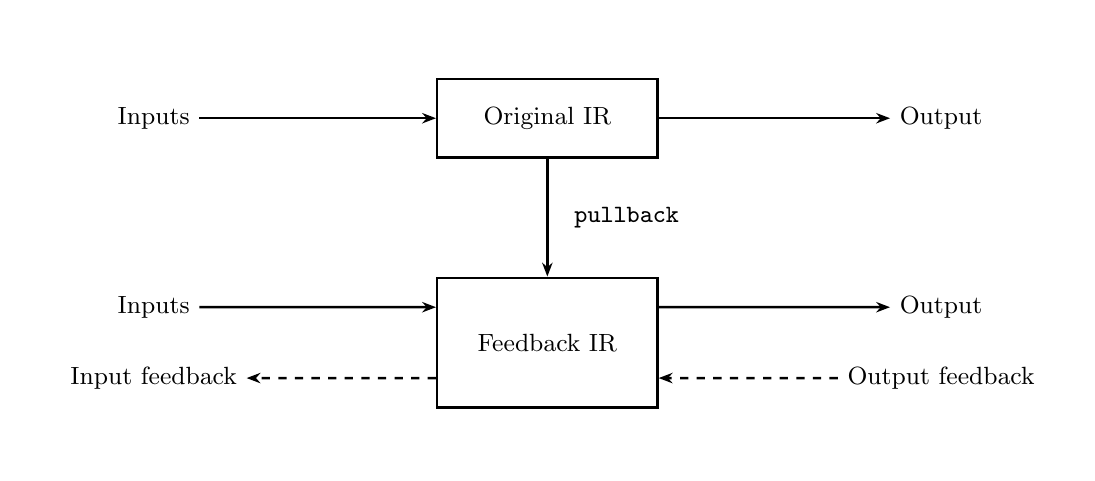
\begin{tikzpicture}[transform panel]
    \transformcanvas

    \node[transform program, minimum height=1.0cm] (original) at (0,1.5) {Original IR};
    \node (inputs) at (-5,1.5) {Inputs};
    \node (output) at (5,1.5) {Output};
    \draw[flow] (inputs.east) -- (original.west);
    \draw[flow] (original.east) -- (output.west);

    \node[transform program, minimum height=1.65cm] (new) at (0,-1.35) {Feedback IR};
    \transformarrow[right]{original.south}{new.north}{\texttt{pullback}}
    \node (newin) at (-5,-0.9) {Inputs};
    \node (changein) at (-5,-1.8) {Input feedback};
    \node (newout) at (5,-0.9) {Output};
    \node (changeout) at (5,-1.8) {Output feedback};
    \draw[flow] (newin.east) -- ([yshift=0.45cm]new.west);
    \draw[flow] ([yshift=0.45cm]new.east) -- (newout.west);
    \draw[feedback] (changeout.west) -- ([yshift=-0.45cm]new.east);
    \draw[feedback] ([yshift=-0.45cm]new.west) -- (changein.east);

\end{tikzpicture}
\end{document}
